\documentclass[12pt,a4paper,french]{article}

\usepackage[T1]{fontenc}
\usepackage[utf8]{inputenc}
\usepackage{fullpage}
\usepackage[french]{babel} 
\usepackage[official]{eurosym}
\usepackage{txfonts}
\usepackage{graphicx}
\usepackage{lastpage}
\usepackage{fancyhdr}
\usepackage{titlesec}
\usepackage{color}
\usepackage{setspace}
\usepackage[nottoc, notlof, notlot]{tocbibind}
\usepackage{hyperref}
\usepackage[french,ruled,vlined]{algorithm2e}
\usepackage{algorithmic}


% Création de la subsubsubsection %
\titleclass{\subsubsubsection}{straight}[\subsection]
\newcounter{subsubsubsection}
\renewcommand\thesubsubsubsection{\thesubsubsection.\arabic{subsubsubsection}}
\renewcommand\theparagraph{\thesubsubsubsection.\arabic{paragraph}}
\titleformat{\subsubsubsection}
  {\normalfont\normalsize\bfseries}{\thesubsubsubsection}{1em}{}
\titlespacing*{\subsubsubsection}
{0pt}{3.25ex plus 1ex minus .2ex}{1.5ex plus .2ex}
\makeatletter
\renewcommand\paragraph{\@startsection{paragraph}{5}{\z@}%
  {3.25ex \@plus1ex \@minus.2ex}%
  {-1em}%
  {\normalfont\normalsize\bfseries}}
\renewcommand\subparagraph{\@startsection{subparagraph}{6}{\parindent}%
  {3.25ex \@plus1ex \@minus .2ex}%
  {-1em}%
  {\normalfont\normalsize\bfseries}}
\def\toclevel@subsubsubsection{4}
\def\toclevel@paragraph{5}
\def\toclevel@paragraph{6}
\def\l@subsubsubsection{\@dottedtocline{4}{7em}{4em}}
\def\l@paragraph{\@dottedtocline{5}{10em}{5em}}
\def\l@subparagraph{\@dottedtocline{6}{14em}{6em}}
\makeatother
\setcounter{secnumdepth}{4}
\setcounter{tocdepth}{4}


\begin{document}

\begin{titlepage}
	\begin{center}
		\begin{spacing}{2}
		{ \Huge{ P.I. : PLANNING INTELLIGENT}}\\[1cm]
		\end{spacing}
		{ \Large{Rapport de mi-projet}}\\[10cm]
		
		\textbf{Auteurs} : 
			Corentin COUDRAY \\
			Christophe JULIEN \\
			Khanh An Noël TRAN \\ 
		\textbf{Groupe} : M2\_9\\
		\textbf{Date} : 13/12/2013\\[2 cm]
	\end{center}	
	% Bas de page %
	\vfill 
	\begin{minipage}[b]{0.3\linewidth}
		
\includegraphics[width=30mm]{logo.png}
	\end{minipage}
	\hfill
	\begin{minipage}[b]{0.3\linewidth}
		{\footnotesize{38 rue Molière}}\\
		{\footnotesize{94200 IVRY sur SEINE}}\\
		{\footnotesize{Tel. : 01 56 20 62 00}}\\
		{\footnotesize{Fax. : 01 56 20 62 52}}\\
		{\footnotesize{http://www.esme.fr}}
	\end{minipage}
\end{titlepage}


\renewcommand{\contentsname}{Sommaire}
\tableofcontents
\newpage

\section{Introduction}

La planification sous contraintes est la discipline des mathématiques appliquées consistant à ordonner diverses séquences ou évènements dans un espace-temps limité. Ces planifications impliquent un grand nombre de contraintes, qu'elles soient liées aux disponibilités de personnes, d'emplacements ou à tout autre type de problème.\\

La réalisation d'une planification est longue et périlleuse. Il est très difficile de concilier l'ensemble des contraintes qui accompagnent cet ordonnancement et de leur organisation manière optimale. La mise en place d'un calendrier est souvent faite à la main ou de manière approximative avec d'autres applications.\\

L'objectif de ce projet est donc de réaliser une application, permettant de générer une planification tenant compte de toutes les contraintes que l'on aura indiquées au préalable. Dans un premier temps, nous nous contenterons de générer un emploi du temps propre à l'école, quitte à élargir notre champ d'action si nous en avons le temps.\\

Ce problème peut être généralisé à toutes les planifications horaires d'employés, comme dans les écoles, les hôpitaux et toutes autres entreprises ayant un roulement de personnel à organiser.

\newpage
\section{Contexte}

Ce sujet a été proposé dans le but d'alléger le travail de M. Maeso. En effet, chaque année, il doit créer manuellement l'intégralité des emplois du temps de l'école, en tenant compte de toutes les contraintes de disponibilités des professeurs, des salles, des élèves et des matières. L'application pourra lui faire gagner un temps non-négligeable dans son travail.

\newpage
\section{Revue littéraire}

Aujourd'hui, il existe déjà des systèmes de planification informatique, mais ils correspondent toujours à des cas bien spécifiques : organisation du personnel médical dans un hôpital, organisation du personnel dans une base militaire, etc. Mais il semble impossible à l'heure actuelle d'imaginer un logiciel générique permettant de lister des contraintes et d'élaborer le planning correspondant et adapté quel que soit le milieu professionnel.

Ainsi, il nous faudra concevoir notre solution dans son ensemble. Nous pourrons tout de même nous inspirer des méthodes de résolution de ces plannings pour essayer de les adapter à notre problème.

En l'occurrence, nous avons trouvé quelques pistes de recherche :
\begin{itemize}
\item Algorithme des colonies de fourmis : cet algorithme est basé sur le comportement réel des fourmis, qui parviennent, par le biais de rétroactions, à trouver le chemin le plus court entre une source de nourriture et leur nid.
\cite{02-algoFourmis}
\item Recherche tabou : cet algorithme consiste à partir d'une position donnée, et à explorer ensuite le voisinage pour choisir la position qui minimise la fonction "objectif". Le mot "tabou" vient du fait qu'une fois une position écartée, nous ne pouvons plus y revenir. Cet algorithme procède donc par élimination jusqu'à trouver une solution convenable.
\cite{03-algoTabou}
\end{itemize}

\paragraph{}
Il existe probablement d'autres algorithmes de ce genre, dont nous aurons besoin pour aboutir à une solution convenable.

\newpage
\section{Cahier des charges}
\subsection{Mise en contexte du problème}

Les algorithmes nécessaires à l'élaboration d'un tel projet relèvent des problèmes dit "NP- complets". Les problèmes NP-complets sont des problèmes qui sont au minimum aussi difficiles que les problèmes NP. Ceux-ci sont des problèmes de décision à temps polynomial.

Cela signifie qu'il n'existe pas de solution exacte, et qu'on ne peut les résoudre avec les méthodes de résolution classiques.

Même s'il n'existe pas de solution déterministe, nous pouvons malgré tout arriver à une solution "acceptable", c'est à dire répondant à l'ensemble des exigences du problème sans pour autant être optimale dans son organisation, en mettant en oeuvre des algorithmes de résolution rétroactifs.

Le temps de résolution de ces problèmes augmente de manière exponentielle par rapport à l'augmentation des paramètres d'entrée. Nous devrons toujours se contenter d'une solution qui sera au mieux "satisfaisante".
\cite{01-npComplet}

\subsection{Langage utilisé}
Nous avons décidé de programmer ce projet en C++ car c'est un langage objet qui nous aidera à mieux organiser notre code, notamment grace au système de classes, au polymorphisme, et l'héritage, etc. De plus, il s'agit d'un langage que nous avons beaucoup pratiqué durant notre cursus.
Le Java répond également à ces critères, mais il est moins rapide, et un langage rapide est primordial pour une résolution raisonnable en temps de notre problème.

\subsection{Simplification du problème}
Le problème étant très conséquent et très complexe, nous avons décidé de réduire le nombre de facteurs à prendre en compte. C'est pourquoi, nous ne nous occupons pas des salles dans un premier temps et nous générons l'emploi du temps sur une seule semaine. Au fur et à mesure que notre solution se consolidera, nous rajouterons de nouveaux paramètres pour le rapprocher petit à petit du cas réel.

\subsection{Interface graphique}
Pour concentrer nos efforts sur la résolution du problème, nous avons également décidé de ne pas inclure l'interface graphique à notre projet, pour des raisons de temps. Cependant, nous pourrons mettre en place une petite interface utilisateur pour le programme qui gèrera les données.

\subsection{Les données d'entrée du problème}
Les données d'entrée du problème sont stockées dans des fichiers externes, car nous estimons que la nature et la quantité des données ne nécessitent pas de base de données. De plus, cela nous permet de vérifier facilement l'exactitude des données saisies lors de l'exécution du programme. Cela nous permet également de ne pas avoir à relancer le programme lorsque nous voulons modifier des données.

Ce système permet également de mettre en place un archivage des données : l'utilisateur n'aura qu'à copier-coller les fichiers dans un dossier séparé.

\subsection{Les données de sortie du problème}
En sortie, chaque classe, professeur et salle auront leur emploi du temps, stockés dans des fichiers externes.

\subsection{Modélisation des données}
\subsubsection{Les professeurs}
Un professeur sera défini par :
\begin{itemize}
\item son nom
\item ses disponibilités
\item la liste des cours qu'il peut enseigner
\end{itemize}

\subsubsection{Les classes}
Une classe sera définie par:
\begin{itemize}
\item son nom
\item le nombre d'élève
\item la liste des cours au programme
\end{itemize}

\subsubsection{Les cours}
Un cours sera défini par:
\begin{itemize}
\item son nom
\item le nombre d'heures de cours
\item le type de salle dans laquelle il doit être donné (un type de cours)
\end{itemize}

\subsubsection{Les salles}
Une salle sera définie par:
\begin{itemize}
\item son nom
\item le nombre de place
\item le type : salle de cours, salle de TP
\end{itemize}

\newpage
\section{Représentation formelle}

\newtheorem{definition}{Définition}
\newtheorem{lemme}{Lemme}
\newtheorem{proposition}{Proposition}
\newtheorem{theoreme}{ThŽorme}
\newtheorem{eg}{Exemple}
\newcommand{\ds}{\displaystyle}



Dans l'ensemble de notre travail, un certain nombre de concepts mathématiques apparaîtront de manière récurrente. Cette section rappelle de façon formelle ces principes\footnote{Il faudrait s'assurer de l'exactitude des différentes définitions}.\\

Soit $\mathbb{E}$ un ensemble et  $\mathcal{R}$ une relation binaire sur les éléments de $\mathbb{E}$. 

\begin{definition}{\emph{Ordre strict : }}
$\mathbb{E}$ muni de $\mathcal{R}$ est une structure d'ordre strict si et seulement si $\mathcal{R}$ est antisymétrique, non réflexive et transitive.\\
\end{definition}

\begin{definition}{\emph{Ordre partiel :} }
$\mathbb{E}$ muni de $\mathcal{R}$ est une structure d'ordre partiel quand une partie seulement des éléments de $\mathbb{E}$ sont soumis à une une relation d'ordre strict.\\
\end{definition}

\begin{definition}{\emph{Préordre :} }
$\mathbb{E}$ muni de $\mathcal{R}$ est une structure de pré-ordre si et seulement si $\mathcal{R}$  est une relation binaire réflexive et transitive.\\
\end{definition}



$(\mathcal{X},\preceq)$ ordre partiel. \\
$(\bigcup\mathcal{X},\prec)$ ordre strict. \\


Le problème de l'organisation l'emploi du temps est la donnée de : 
\begin{enumerate}
\item Un ensemble de matières (une promotion) $\mathcal{X}:=\{X_{1},\dots, X_{n}\}$ muni d'un ordre partiel $\mathcal{O}$. \item Un ensemble de blocs ordonnés (ordre strict) $W$ correspondant à un ensemble de semaines de cours. Nous sommes convenus que $|W|:=k22$.\footnote{Considérant qu'un bloc est composé de quatre heures consécutives et considérant qu'une semaine est une juxtaposition de 22 blocs.}
\item Un élément $X_{i_{i\in\overline{1,n}}}\in\mathcal{X}$ est un ensemble de cours muni d'un ordre strict sur des blocs de quatre heures quelle que soit la matière .i.e. quels que soient $i$, $i'$, deux indices de matière, et $j$, $j'$ deux indices de cours, nous avons $x_{i,j} \prec x_{i',j'}$ ou $x_{i,j} \succ x_{i',j'}$


\end{enumerate} 

\paragraph{Tâche : } Déterminer un ordre des $x_{i,j}$ ($i$ correspond un indice de matière, $j$ un indice de cours de la matière $X_{i}$) tel que les propriétés suivantes soient respectées.
\begin{itemize}
\item Tous les cours soient placés au sein des $k22$ blocs.
\item l'ordre partiel sur les matières soit respecté
\item l'ordre partiel sur les cours soit respecté
\item un cours ne peut avoir lieu plus d'une fois une même semaine quelle que soit la matière.
\item un cours occupe un même bloc sur l'ensemble des $k22$ blocs.
\end{itemize}   

Nous introduisons un niveau de conflit compris entre $1$ et $n$. Il représente le nombre de profs disponibles pour enseigner une matière donnée\footnote{ce niveau de conflit peut vraisemblablement concerner les salles aussi}.

\newpage
\section{Les acteurs}        
Il existe deux principaux types d'acteur pour notre logiciel:

\subsection{Premier acteur : Saisie des données}
Le rôle du premier acteur est de saisir toutes les données relatives aux professeurs, salles, et élèves, et tous les paramètres nécessaires à la génération de l'emploi du temps.
        
\subsection{Second acteur : Maintenance de l'emploi du temps}
Etablir un emploi du temps est une bonne chose, mais il faut  également pouvoir le modifier au cours de l'année si des évènements imprévus doivent être rajoutés.
Le rôle du deuxième acteur est donc de gérer la maintenance de l'emploi du temps au fur et à mesure que l'année avance. Il doit pouvoir rajouter des évènements dans l'emploi du temps des professeurs et/ou des élèves.


\newpage
\section{Cas d'utilisation}
\subsection{Génération de l'emploi du temps}    
\begin{figure}[! ht ]
    \centering
    \begin{minipage}[t]{14 cm}
        \centering
            \fbox{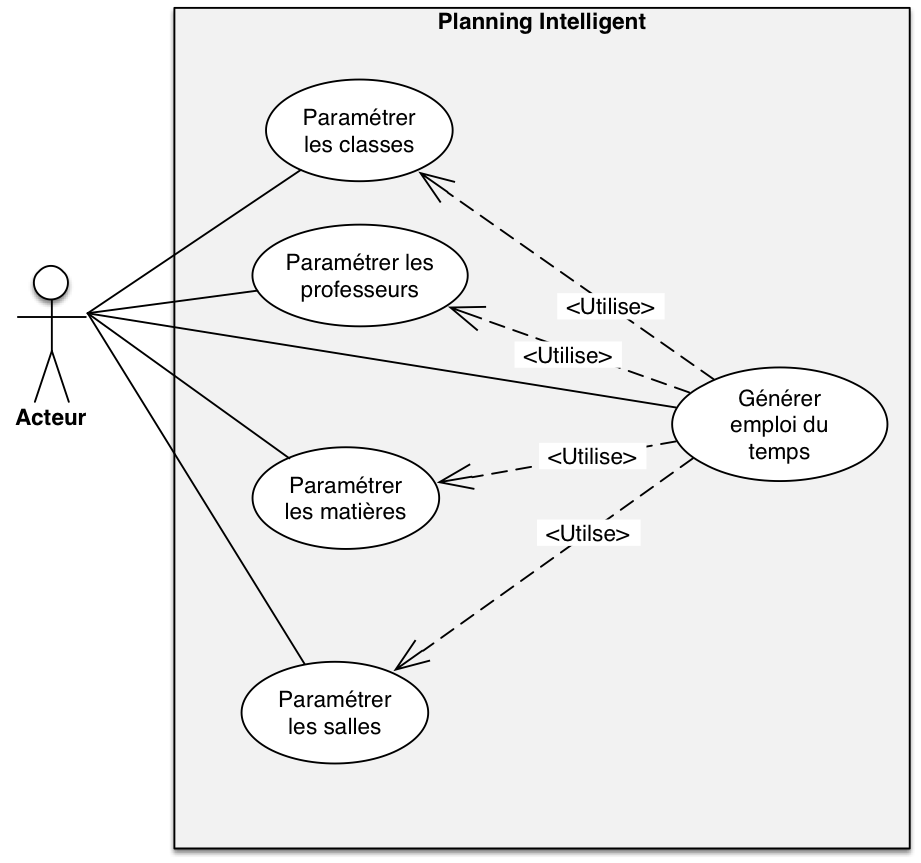
\includegraphics[width=140mm, height=140mm]{CasUtilisation1.png}}
        \caption {Diagramme de cas d'utilisation, génération de l'emploi du temps}
    \end{minipage}
\end{figure}
            
\subsubsection{Objectif}
L'objectif est de créer un emploi du temps à partir de données brutes entrées par l'utilisateur.

\subsubsection{Acteurs}
L'acteur est celui qui est chargé de la saisie des données.
        
\subsubsection{Données échangées et description des enchaînements}    
L'acteur en question entre les différentes données propres aux professeurs, classes, salles, et matières. Pour chaque élément, il devra remplir des critères bien spécifiques:

\begin{itemize}
\item Pour chaque professeur, il doit entrer son nom, les matières que celui-ci enseigne et ses disponibilités dans la semaine. 
\item Pour chaque matière, il doit entrer le nom de la matière, le programme qui devra être dispensé au cours de l'année (matières et nombre d'heures).
\item Pour chaque classe, il doit préciser le nom de la classe, la promotion à laquelle elle appartient et le nombre d'élève que contient cette classe.
\item Pour chaque salle, il doit entrer leur contenance et leur type (salle de TP info, salle de cours, etc.)
\end{itemize}
                    
Une fois que toutes les données ont été entrées, le logiciel génère tous les emplois du temps de l'école. 
        
\newpage
\subsection{Maintenance de l'emploi du temps}    
\begin{figure}[! ht ]
    \centering
    \begin{minipage}[t]{14 cm}
        \centering
        \fbox{
            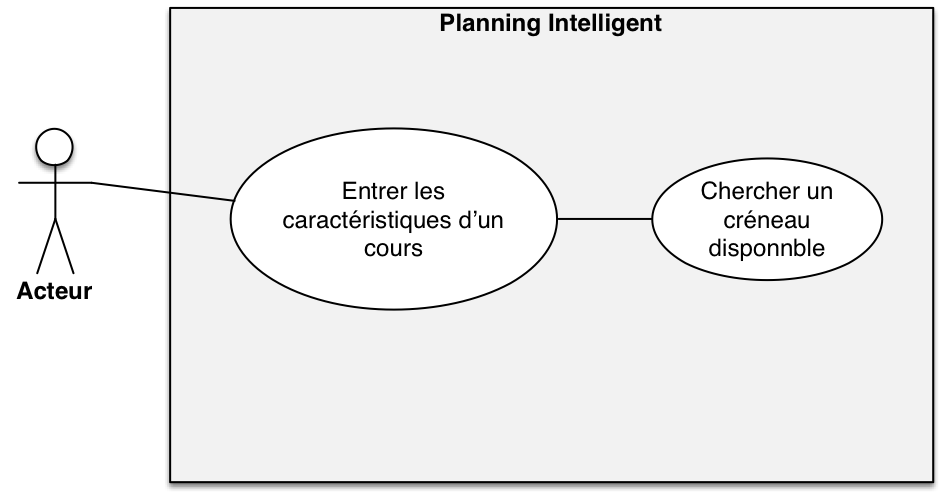
\includegraphics[width=140mm, height=80mm]{CasUtilisation2.png}
        }
        \caption {Diagramme de cas d'utilisation, maintenance de l'emploi du temps}
    \end{minipage}
\end{figure}
            
\subsubsection{Objectif}
Pour une raison ou pour une autre, l'utilisateur peut être amené à rajouter un évènement dans l'emploi du temps. Le logiciel doit donc le permettre en tenant  compte des évènements déjà placés et des contraintes que cela implique, sans avoir à générer à nouveau la totalité de l'emploi du temps. 
                
\subsubsection{Acteurs}
Le seul acteur à intervenir dans ce cas est celui chargé de la maintenance.
            
\subsubsection{Données échangées}
Pour placer un cours dans l'emploi du temps, le programme consulte les disponibilités de chaque élément:

\begin{itemize}
\item Les disponibilités des professeurs ou des intervenants
\item Les disponibilités des élèves
\item Les disponibilités d'une salle convenant à l'évènement, et dont la capacité est suffisante pour accueillir tous les élèves.
\end{itemize}
                
\subsubsection{Description des enchaînements}        
\subsubsubsection{Pré-condition}
Lorsque l'utilisateur désire rajouter un évènement, il lui faut connaître les disponibilités de chaque entité, et savoir quelles classes sont concernées par l'évènement, si elles doivent recevoir l'évènement par classe ou par promo, etc.

\subsubsubsection{Séquence}
L'utilisateur entre les disponibilités de chacun dans le programme, et celui-ci cherche les différents créneaux possibles pour placer le cours. L'utilisateur a alors deux possibilités : soit il laisse le programme placer automatiquement le cours, soit il demande au programme d'afficher la liste des créneaux disponibles afin de placer manuellement le cours. Celui-ci n'a alors qu'à choisir le créneau qui lui semble le plus adapté.

\newpage
\section{Organisation des données}
Nous avons défini la semaine sur 22 créneaux de 2 heures chacun. Avec 2 créneaux le matin et 2 l'après-midi du lundi au samedi matin.

\subsection{Les professeurs}
Les disponibilités du professeur sont représentées par un mot binaire de 22 bits, un bit par créneau. 1 représentant une disponibilité et 0 une indisponibilité.
Le mot binaire d'un professeur correspond à une semaine : chaque nouvelle semaine aura un nouveau mot binaire.

Lorsque nous ajoutons un cours à un professeur, ses disponibilités sur la semaine concernée changent, et il faut donc modifier le mot binaire en conséquence.


\subsection{Les classes}
Une classe comprend une liste de semaines, représentant le semestre ou l'année. Celles-ci possèdent un numéro (ID) définissant leur ordre d'arrivée dans l'année, et 22 créneaux assignés que l'on doit remplir avec les cours planifiés à la classe.

Chaque classe possède également un nombre d'élèves déterminant la taille minimum de la salle dans laquelle se déroulera le cours.

Chaque classe a une liste de cours qu'elle devra obligatoirement suivre.

\subsection{Les matières}
Une matière est définie par son nom, la promotion à laquelle elle est rattachée, et le nombre d'heures à enseigner. Dans le cas d'une matière commune à plusieurs promotions, nous les distinguons par des noms différents : un pour chacune des promotions (ex: Algèbre B1, Algèbre B2).

De la même manière, nous distinguons les cours en classe entière, des cours en demi-groupes et des TPs.
Cela implique un dernier paramètre qui détermine le type de salle dans laquelle la matière doit être enseignée (ex: un TP ne peut pas être fait dans un amphithéâtre).

\subsection{Les salles}
Une salle est définie par son nom, sa capacité (nombre de places), et son type.
La capacité est un paramètre déterminant dans le choix de la salle à attribuer lors du placement d'un cours dans l'emploi du temps.

De même, le type de la salle va de pair avec le type d'une matière explicité précédemment. Ces deux paramètres doivent concorder pour que la salle puisse être attribuée à un cours.

Enfin, il faut également préciser dans quel bâtiment se trouve la salle: dans les locaux d'Ivry-sur-Seine, ou dans ceux de Montparnasse, car comme expliqué précédemment, les professeurs ne peuvent pas se permettre de donner de cours dans les deux locaux lors d'une même demi-journée.

\subsection{Les semaines}
Chaque entité de notre emploi du temps (classes, professeurs, salles) doit être organisée dans le temps. Il faut donc leur attribuer un paramètre 'semaine', correspondant à leur planning d'occupation.
Ces semaines sont être mises à jour à chaque fois qu'un nouveau cours sera ajouté au planning.

\subsection{Les fichiers externes}
Les données d'entrée à stocker dans les fichiers sont toutes celles que l'utilisateur devra saisir pour lancer le programme. C'est à dire les données sur les professeurs (nom, disponibilités, matières), sur les matières (nom, nombre d'heures, promotions associées) et les salles (nom, capacité, type, bâtiment).\\

Chaque type de donnée est stockée dans un fichier séparé. Au sein du fichier, une ligne contient tous les paramètres d'un seul élément. Les données seront donc récupérées lignes par ligne à chaque exécution du programme.\\

Les données en sortie du problème, c'est à dire les emplois du temps de chaque éléments (classes, profs, salles) seront également dans des fichiers externe.

\subsection{Diagrammes de classes}
Ce diagramme représente les liens entre les différentes classes de notre programme avec les simplifications que nous avons décidé de réaliser dans un premier temps.\\
\begin{figure}[! ht ]
    \centering
    \begin{minipage}[t]{14 cm}
        \centering
            \fbox{
                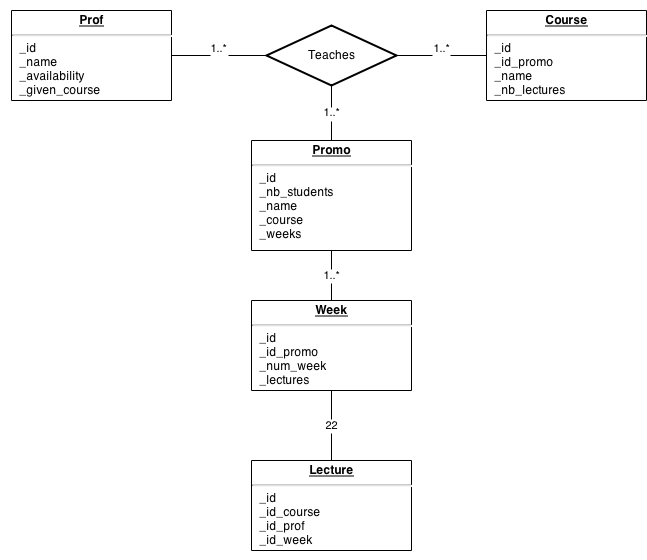
\includegraphics[width=120mm, height=110mm]{DiagrammeClasse1.png}
            }
        \caption {Diagramme de classes de mi-projet}
    \end{minipage}
\end{figure}

\paragraph{}
Le bloc "Teaches" représente les relations de $n$ à $n$ entre 
\begin{itemize}
\item les professeurs("Prof") et les matières("Course") : 
	\begin{itemize}
	\item[$\bullet$] un professeur peut enseigner plusieurs matières
	\item[$\bullet$] une matière peut être enseignée par plusieurs professeurs
	\end{itemize}
\item les promotions ("Promo") et les professeurs :
	\begin{itemize}
	\item[$\bullet$] une promotion a plusieurs professeurs
	\item[$\bullet$] un professeur enseigne à plusieurs promotions
	\end{itemize}
\item les matières et les promotions : 
	\begin{itemize}
	\item[$\bullet$] une promotion a plusieurs matières
	\item[$\bullet$] une matière est enseignée à plusieurs promotions
	\end{itemize}
\end{itemize}


\paragraph{}
Ce second diagramme est une ébauche du diagramme des classes final sous réserve de modifications lorsque nous ajouterons les salles à notre problème.\\

\begin{figure}[! ht ]
    \centering
    \begin{minipage}[t]{14 cm}
        \centering
            \fbox{
                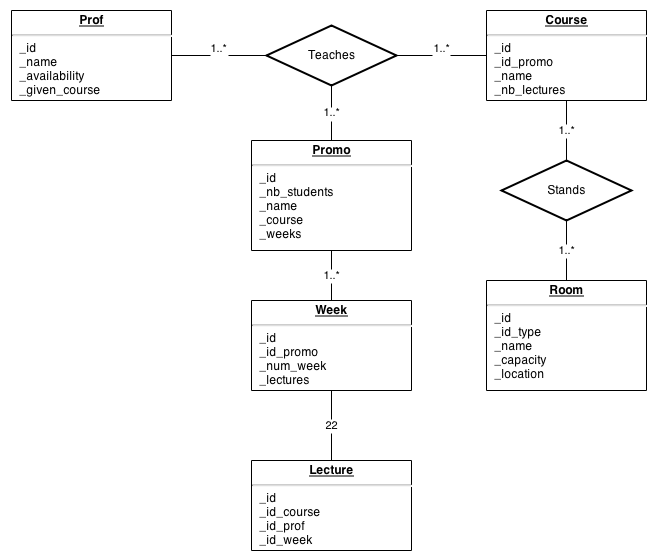
\includegraphics[width=120mm, height=110mm]{DiagrammeClasse2.png}
            }
        \caption {Diagramme de classes final envisagé}
    \end{minipage}
\end{figure}

\paragraph{}
Le bloc "Stands" représente les relations de $n$ à $n$ entre les matières ("Course") et les salles de cours ("Room"):
\begin{itemize}
\item une matière peut être enseignée dans plusieurs salles
\item une salle peut recevoir plusieurs matières
\end{itemize}

Chaque salle va avoir un type spécifique correspondant aux différents types de cours (cours classe entière, TP, cours de demi classe).

\newpage
\section{Etapes de résolution}
\subsection{Simplification du problème}
Comme expliqué précédemment, nous avons décidé de commencer notre projet en le réduisant au maximum, puis nous rajouterons des paramètres au fur et à mesure que le projet avance afin de se rapprocher petit à petit des conditions réelles.\\

Cette manière de procéder nous permet de nous concentrer sur une seule contrainte à la fois, et donc d'optimiser la résolution de celle-ci.\\

Nous allons donc commencer par considérer le cas d'une promotion, avec une seule classe, sur un semestre.\\

Le problème peut alors se fragmenter en plusieurs points :
\begin{itemize}
\item répartir l'ensemble des cours sur les différentes semaines du semestre
\item répartir les cours sur les différents créneaux d'une semaine
\item éviter que plusieurs cours se superposent : 
	\begin{itemize} 
	\item[$\bullet$] une classe ne doit pas recevoir plus d'un cours sur un même créneau
	\item[$\bullet$] plusieurs professeurs ne peuvent pas donner de cours sur un même créneau
	\end{itemize}
\item tenir compte des disponibilités des professeurs et de la classe lors de l'attribution d'un nouveau cours
\item répartir en priorité les professeurs dont les disponibilités sont les moindres
\item mettre à jour les disponibilités de chaque protagoniste dès l'ajout d'un cours
\item lorsqu'un cours est présent sur plusieurs semaines consécutives, il doit se retrouver sur le même créneau.
\end {itemize}

\subsection{Considération de l'ensemble des classes d'une promotion}
Lorsque nous aurons trouvé l'algorithme répondant à ces critères, nous pourrons considérer toutes les classes de la promotion.\\

De nouvelles contraintes se posent :
\begin{itemize}
\item un professeur ne peut pas dispenser un même cours à deux classes différentes sur un même créneau
\item vérifier que pour une matière donnée, l'ensemble des créneaux des professeurs qualifiés soit suffisant pour donner tous les cours
\item la répartition du programme doit être homogène : toutes les classes doivent recevoir les mêmes cours sur une même semaine
\end{itemize}

\subsection{Considération de l'ensemble des promotions}
Ensuite nous pourrons considérer la totalité des promotions. Il n'y a pas réellement de nouvelle contrainte, mais c'est à ce stade que l'algorithme de résolution va réellement être mis à l'épreuve, et que le temps d'exécution du programme va vraiment augmenter.

\subsection{Considération des salles}
Nous rajoutons ensuite la contrainte des salles. Ce nouveau paramètre va énormément compliquer le problème :
\begin{itemize}
\item vérifier qu'une salle ne reçoit qu'un seul cours par créneau
\item vérifier qu'une salle a la capacité suffisante pour accueillir tous les élèves d'un cours donné
\item vérifier qu'une salle contient les équipements adaptés au cours
\end{itemize}

\subsection{Cas réel}
Enfin, les enseignants de l'ESME peuvent dispenser des cours dans les locaux d'Ivry-sur-Seine et de Montparnasse. Pour des raisons de timing, les professeurs ne doivent pas avoir de cours à donner dans les deux locaux sur une même demi-journée. Il faut donc introduire ce paramètre dans l'attribution des cours, ce qui va restreindre davantage le nombre de solutions du problème.

\newpage

\documentclass[12pt,a4paper,french]{article}

\usepackage[T1]{fontenc}
\usepackage[latin9]{inputenc}
\usepackage{fullpage}
\usepackage[french]{babel} 
\usepackage[official]{eurosym}
\usepackage{txfonts}
\usepackage{graphicx}
\usepackage{lastpage}
\usepackage{fancyhdr}
\usepackage{titlesec}
\usepackage{color}
\usepackage{setspace}
\usepackage[nottoc, notlof, notlot]{tocbibind}
\usepackage{hyperref}
\usepackage[french,ruled,vlined]{algorithm2e}
\usepackage{algorithmic}

\begin{document}

\title{Algorithmes -- Emploi du temps}
\author{Coudray -- Julien -- Tran}
\date{\today}
\maketitle

\section{Pré-traitements}
Avant de réaliser l'emploi du temps, le programme procède à des vérifications sur les données d'entrées afin de détecter toutes les incohérences. Ainsi, il élimine au préalable une partie des traitements qui n'aboutiront pas.

\subsection{Le nombre de professeur}
La première vérification concerne le nombre de professeurs en entrée. Nous vérifions s'il y a assez de professeurs pour dispenser les cours de chaque classe.
Ainsi pour un cours donné, l'algorithme somme les disponibilités des professeurs puis compare le résultat au nombre de classe.\\
Si le cours est sur 4 heures, alors la somme des disponibilités est divisée par 2. En effet, le cours en question nécessite deux créneaux consécutifs pour être dispensé.\\

Soit $n$ le nombre de professeurs pouvant donner un cours $c$ et $m$ le nombre de classe devant suivre ce cours.
Pour un cours de 2 heures, nous avons:
\begin{center}
$\sum_{i=0}^n dispo_{prof_i} > m$
\end{center}

Pour un cours de 4 heures, nous avons: 
\begin{center}
$\frac{\sum_{i=0}^n dispo_{prof_i}}{2} > m$
\end{center}

L'opération est répétée pour l'ensemble des cours. 

\begin{algorithm}
\caption{Pré-traitement nombre de professeurs}
\begin{algorithmic}
\FORALL{$Courses$}
\STATE $idCourse \leftarrow$ identifiant de $Courses$
\STATE $idPromo \leftarrow$ identifiant de la promotion recevant $Courses$
\STATE $nbClasses \leftarrow$ nombre de classe de la promotion $idPromo$
\FORALL{$Profs$}
\IF {$Profs$ donne le cours $idCourse$}
\FORALL {$CreneauxProf$}
\IF {$Profs$ est disponible}
\STATE $nbCreneaux \leftarrow nbCreneaux + 1$
\ENDIF
\ENDFOR
\ENDIF
\ENDFOR
\IF {$Courses$ est sur 4h}
\STATE $nbCreneaux \leftarrow nbCreneaux / 2$
\ENDIF
\IF{$nbClasses > nbCreneaux$}
\STATE display (Erreur sur le nombre de professeur pour la promo $idPromo$)
\STATE EXIT FAILURE
\ENDIF
\ENDFOR
\STATE display (Nombre de professeurs ok)
\end{algorithmic}
\end{algorithm}

\newpage

\subsection{Le nombre de cours total sur le semestre}
La seconde vérification porte sur le nombre d'heures de cours à dispenser à une classe. Ce nombre ne doit pas excéder la totalité des heures du semestre. Le programme somme l'ensemble des cours que possède une classe et le compare au nombre d'heures du semestre.

Soit $n$ le nombre de cours d'une classe $p$, $s$ le nombre de semaines sur un semestre, $c$ le nombre de créneaux sur une semaine et $h$ le nombre d'heures d'un créneau: 

\begin{center}
$\sum_{i=0}^n nbHeures_{cours_i} \leq s*c*h$
\end{center}

\begin{algorithm}
\caption{Pré-traitement nombre d'heures sur le semestre}
\begin{algorithmic}
\FORALL{$Classes$}
\STATE $listCourses \leftarrow$ ensemble des cours que suit une classe
\FORALL {$courses$ in $listCourses$}
\STATE $nbHours \leftarrow nbHours +$ nombre d'heures du cours $courses$
\ENDFOR
\IF {$nbHours$ > (nombre de semaines du semestre * nombre de créneaux par semaine * nombre d'heures par créneau)}
\STATE display(Erreur, trop d'heures pour la classe $Classes$)
\STATE EXIT FAILURE
\ENDIF
\ENDFOR
\STATE display(Nombre d'heures de cours ok)
\end{algorithmic}
\end{algorithm}

Une fois ces pré-traitements réalisés, nous pouvons commencer la conception de l'emploi du temps de l'école.

\newpage
\section{Réalisation de l'emploi du temps}
La réalisation de l'emploi du temps se déroule en deux étapes qui sont réalisées indépendamment pour chaque promotion. Chaque classe d'une promotion suit le même programme avec la même liste d'enseignants potentiels.
C'est pourquoi chaque promotion va avoir un emploi du temps sur le semestre. A savoir, la planification des cours indiquant la semaine de début et de fin.
Enfin, un emploi du temps final sera réalisé semaine par semaine avec chaque cours placés sur ses créneaux respectifs.
\begin{algorithm}
\caption{Principe général de conception des emplois du temps}
\begin{algorithmic}
\FORALL{$Promo$}
\STATE $idCourses \leftarrow$ liste de tous les cours que doivent suivre la promotion $Promo$
\STATE repartitionCoursSemestre($idCourses, programmeSemestre$)
\STATE repartitionCoursPromotions($Promo, programmeSemestre$)
\ENDFOR
\end{algorithmic}
\end{algorithm}

\subsection{Répartition du programme sur le semestre}
La première étape de l'algorithme de résolution est de répartir de l'ensemble du programme de chaque promotion sur le semestre. Cette étape consiste à indiquer pour chaque cours la date de début et de fin semaine.\\

La répartition se déroule en deux étapes : 
\begin{itemize}
\item Le trie des cours 
\item Le placement des cours sur le semestre\\
\end{itemize}

L'objectif est de répartir au mieux les cours sur le semestre. Il faut donc réussir à placer le maximum de cours les uns à la suite des autres. C'est pourquoi nous plaçons les cours les plus longs en premier, puis nous vérifions s'il est possible de placer un nouveau cours derrière ceux-là, sinon nous le plaçons en début de semestre.\\

Un cours de 4 heures impose plus de contraintes. En effet, il s'agit d'un cours où le professeur et la classe doivent avoir deux créneaux consécutifs dans la même demi-journée. C'est pourquoi un cours de 4 heures doit être planifié sur le semestre avant un cours de 2 heures.\\

Pour se faire, les cours vont être séparés en deux listes : une pour les cours de 4 heures et une autre pour les cours de 2 heures. Ainsi pour chacunes des listes, un trie décroissant est effectué par rapport au nombre de semaines sur lequel les cours vont être suivis.\\

$semaineDebut_{coursPlace} + nbSemaine_{coursPlace} + nbSemaine_{nouveauCours} \leq nbSemaine_{semestre}$\\

Chaque élément du semestre va avoir les informations suivantes :
\begin{itemize}
\item L'identifiant du cours
\item Le numéro du début de la semaine
\item Le nombre de semaine du cours
\item Le cours qui le suit
\end{itemize}

\begin{algorithm}
\caption{Algorithme principale de la répartition des cours sur le semestre}
\begin{algorithmic}
\REQUIRE liste $idCourse$, liste $programmeSemestre$
\FORALL {$idCourse$}
\IF {$idCourse$ est un cours sur 2h}
\STATE $idCourses2 \leftarrow$ pushback $idCourses$
\ELSE
\STATE $idCourses4 \leftarrow$ pushback $idCourses$
\ENDIF
\ENDFOR
\STATE Trie de $idCourses2$ par nombre de semaine de cours décroissant
\STATE Trie de $idCourses4$ par nombre de semaine de cours décroissant
\STATE $idCourses$ est vider
\STATE $idCourses \leftarrow$ pushback $idCourses4$
\STATE $idCourses \leftarrow$ pushback $idCourses2$
\STATE $programmeSemestre \leftarrow$ repartitionDesCours($idCourses$)
\end{algorithmic}
\end{algorithm}

\begin{algorithm}
\caption{repartitionDesCours($idCourses$)}
\begin {algorithmic}
\REQUIRE liste $idCourses$ triée par nombre de semaine d'un cours et par cours de 4H et 2H
\STATE initialisation de $coursProgrammes$
\FORALL {$idCourses$}
\FORALL {$coursProgrammes$}
\IF {$programmeSemestre$ a cours placé}
\STATE checkNextCourse($idCourses, coursProgrammes$)
\IF {$idCourses$ a été programmé}
\STATE $coursPlace \leftarrow true$
\STATE BREAK
\ENDIF
\ENDIF
\ENDFOR
\IF {$coursPlace == false$}
\STATE $coursProgrammes \leftarrow$ pushback $idCourses$ en début de semestre
\ENDIF
\ENDFOR
\RETURN $coursProgrammes$
\end{algorithmic}
\end{algorithm}

\begin{algorithm}
\caption{checkNextCourse($idCourses, coursProgrammes$)}
\begin {algorithmic}
\IF {$coursProgrammes$ a un cours après lui déja}
\STATE checkNextCourse($idCourses, coursProgrammes$ du cours suivant)
\ELSIF {$semaineDebut_{coursProgrammes} + nbSemaine_{coursProgramme} + nbSemaine_{idCourses} \leq nbSemaine_{semestre}$}
\STATE $coursProgramme \leftarrow$ pushBack $idCourses$
\ENDIF
\end{algorithmic}
\end{algorithm}



\end{document}

\section{Discussions}

Le problème étant vraisemblablement Np-difficile, nous doutons de la possibilité d'établir un algorithme de résolution exacte dans un temps raisonnable, étant donnée la taille des instances que nous avons observées. Nous avons considéré qu'une approche heuristique (voire métaheuristique), offrant une solution réalisable mais non nécessairement optimale, serait plus appropriée pour des raisons pratiques évidentes.\\

Par ailleurs, au regard du nombre de contraintes associées au problème, nous devrons commencer par une définition simplifiée d'une "instance" du problème, en écartant un maximum de contraintes pour établir un cadre de résolution théorique clair : nous l'enrichirons tout au long de notre projet. La version tant théorique que logicielle présentée dans ce rapport reflète l'état de notre avancée et est de ce fait partielle.\\

\newpage
\section{Conclusion}

Jusqu'à maintenant, nous avons mis en place un système permettant à l'utilisateur de saisir les données : il les rentre une à une dans la console, et elles sont automatiquement ajoutées dans un fichier externe. Celles-ci sont alors mises en relation par le programme au sein d'une architecture bien définie.\\

Pour des raisons pratiques, nous avons décidé de réduire le nombre de contraintes à considérer de manière à commencer avec une instance plus simple du problème.\\

Nous avons également réalisé une ébauche du traitement de placement d'un cours. Pour cela, nous effectuons un pré-traitement permettant d'écarter les associations qui n'aboutiront pas pour éviter les calculs inutiles.\\

Ainsi, toute l'architecture permettant la modélisation de l'emploi du temps est faite. Il nous faut maintenant mettre en place les algorithmes qui mèneront à l'ordonnancement des multiples éléments de l'école. Nous pourrons alors établir les différents emplois du temps. Pour se faire, il n'y aura qu'à modéliser les données de sortie.\\

Enfin, le programme nécessitera des fonctions de maintenance pour mettre à jour l'emploi du temps tout au long de l'année.


\newpage
\addcontentsline{toc}{section}{Table des figures}
\listoffigures

\newpage
\bibliographystyle{unsrt}
\bibliography{biblio}


\end{document}